\documentclass[a4paper]{article}

%% Language and font encodings
\usepackage[english]{babel}
\usepackage[utf8x]{inputenc}
\usepackage[T1]{fontenc}

%% Sets page size and margins
\usepackage[a4paper,top=3cm,bottom=2cm,left=3cm,right=3cm,marginparwidth=1.75cm]{geometry}

%% Useful packages
\usepackage{amsmath}
\usepackage{graphicx}
\usepackage[colorinlistoftodos]{todonotes}
\usepackage[colorlinks=true, allcolors=blue]{hyperref}
\usepackage{float}
\usepackage{algorithm}
\usepackage[noend]{algpseudocode}
\usepackage{listings}

\usepackage{color}

\definecolor{dkgreen}{rgb}{0,0.6,0}
\definecolor{gray}{rgb}{0.5,0.5,0.5}
\definecolor{mauve}{rgb}{0.58,0,0.82}
\definecolor{darkblue}{rgb}{0.0,0.0,0.6}
\definecolor{cyan}{rgb}{0.0,0.6,0.6}

 \lstset{frame=tb,
  language=C++,
  breaklines=true,
  showstringspaces=false,
  columns=flexible,
  numbers=none,
  commentstyle=\color{dkgreen},
  stringstyle=\color{mauve},
  tabsize=3
}
\lstdefinelanguage{XML}
{
  morestring=[b]",
  morestring=[s]{>}{<},
  morecomment=[s]{<?}{?>},
  stringstyle=\color{black},
  identifierstyle=\color{darkblue},
  keywordstyle=\color{cyan},
  morekeywords={xmlns,version,type,ma-id}% list your attributes here
}

\graphicspath{ {images/} }

\title{Peg Solitaire Backtracking Assignment}
% \author{}
% Update supervisor and other title stuff in title/title.tex

\begin{document}
\begin{titlepage}

\newcommand{\HRule}{\rule{\linewidth}{0.5mm}} % Defines a new command for the horizontal lines, change thickness here

\center % Center everything on the page
 
%----------------------------------------------------------------------------------------
%	HEADING SECTIONS
%----------------------------------------------------------------------------------------

\textsc{\LARGE University of the Witwatersrand}\\[1.5cm] % Name of your university/college
\textsc{\Large COMS3005: Advanced Analysis of Algorithms}\\[0.5cm] % Major heading such as course name
% \textsc{\large Minor Heading}\\[0.5cm] % Minor heading such as course title

%----------------------------------------------------------------------------------------
%	TITLE SECTION
%----------------------------------------------------------------------------------------
\makeatletter
\HRule \\[0.4cm]
{ \huge \bfseries \@title}\\[0.4cm] % Title of your document
\HRule \\[1.5cm]
 
%----------------------------------------------------------------------------------------
%	AUTHOR SECTION
%----------------------------------------------------------------------------------------
{\large \today}\\[2cm] % Date, change the \today to a set date if you want to be precise

\begin{minipage}{1\textwidth}
  \Large \emph By Bancroft, E. (879192)\\
  \Large \emph And Chalom, J. (711985)\\
\end{minipage}

% If you don't want a supervisor, uncomment the two lines below and remove the section above
%\Large \emph{Author:}\\
%John \textsc{Smith}\\[3cm] % Your name

%----------------------------------------------------------------------------------------
%	DATE SECTION
%----------------------------------------------------------------------------------------



%----------------------------------------------------------------------------------------
%	LOGO SECTION
%----------------------------------------------------------------------------------------

% \includegraphics[width=8cm]{title/logo.png}\\[1cm] % Include a department/university logo - this will require the graphicx package
 
%----------------------------------------------------------------------------------------

\vfill % Fill the rest of the page with whitespace

\end{titlepage}

% \lfoot{School of Computer Science and Applied Mathematics}
\clearpage
\setcounter{page}{1}
% \setcounter{section}{1}
\pagenumbering{arabic}

% \section*{Abstract}


\section{Introduction}
Our aim for this assignment is to implement a version of the Peg solitaire game and use the backtracking algorithm to find solutions to randomly generated peg positions of the game. We have analyzed the complexity of our solution algorithm and performed empirical analysis on our implementation.

\section{Background}
Peg Solitaire is a board game which has a number of holes that can be filled with pegs. We have chosen to use the European (French) style of board which has four extra positions for pegs on the board \ref{board}. This style has 37 peg holes. The aim of the game is to remove pegs until only one peg remains. There are 3 terminal win states in our chosen configuration \ref{board}. Moves are made when pegs jump over a peg and are placed in an open position. Then the peg which has been jumped over, is removed. This move can happen in both horizontal and vertical directions. Its is possible to hit sub-optimal states where there are more pegs left on the board but no possible moves left \cite{harder}. 

% Have example moves and sub-optimal states?
\begin{figure}[H]
	\centering
	\label{board}
	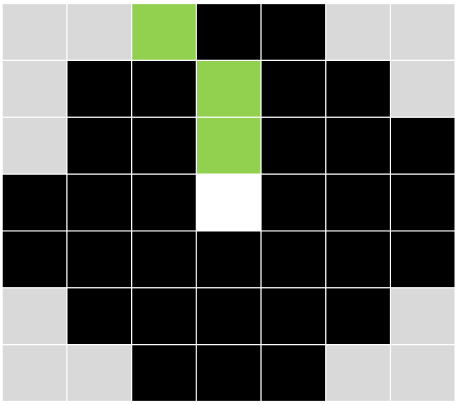
\includegraphics[width=.50\textwidth,scale=.50]{images/board}
	\caption{Diagram of an European Peg Solitaire Board Where the
				Black Squares Represent Peg Positions,
				Green Are Terminal Positions,
				Grey Are Not Positions and
				White is the Central Pixel.
			}
\end{figure}

% cite the way-back machine??
\noindent The backtracking algorithm is similar to a brute force approach to finding solutions to problems but is more systematic. It attempts to follow a logical series of decisions in solving these problems and when a block state occurs the algorithm will backtrack to previous decisions and choose different paths until a terminal (complete) state is reached. The full set of solutions to a problem can be found by continuing to run the algorithm until all paths have been searched but that is not always necessary.

\begin{algorithm}[H]
	\begin{algorithmic}[1]
		\Procedure{FindSolution}{\texttt{start, final, path}}
			\If {\texttt{start.numPegs <= final.numPegs}}
				\State \Return (start = final)
			\Else 
				\For{\texttt{each jump $J \in$ [0,n) x [0,m) x \{NORTH,EAST,SOUTH,WEST\}}}
			        \If {$J$ is a legal jump for start}
			        	\State \texttt{start.makeMove($J$)}
			        	\State \texttt{path.push($J$)}
			        	\State \texttt{found = FindSolution(start, final, path)}

			        	\If {found}
			        		\State \Return {TRUE}
			        	\Else
			        		\State \texttt{start.makeReverseMove($J$)}
			        		\State \texttt{path.pop()}
			        	\EndIf
					\EndIf
		      	\EndFor
		      	\State \Return{FALSE}
			\EndIf 
		\EndProcedure
	\end{algorithmic}
	\caption{Recursive Algorithm (From References \cite{lab5})}\label{euclid}
\end{algorithm}


\subsection{Stack Based Algorithm}
The stack based algorithm we used is adapted from the recursive version. The purpose of implementing the stack based algorithm was to compare it's effciency to that of the recursive based algorithm. The recursive algorithm was also expected to be much slower and perhaps unable to test all the given amount of peg positions in a resonable test time.

\begin{algorithm}[H]
	\begin{algorithmic}[1]
		\Procedure{FindSolution}{\texttt{start, outPath, totalNumPegs, numValidMoves}}
			\State currentState $\leftarrow$ start
			\State path $\leftarrow$ start.getMoves()
			\State numPegs $\leftarrow$ currentState.getNumPegs()
			\State found $\leftarrow$ FALSE
			\State i $\leftarrow$ 1

			\State stackVector.push(path)
			\State boardVector.push(currentState)

			\While {found is FALSE and i <= numPegs and stackVector.size() > 0 and path.size() > 0}
				\State path $\leftarrow$ stackVector.pop()
				\State currentState $\leftarrow$ boardVector.pop()

				\While {\texttt{currentState.checkGameEnd() != FALSE}}
					\State numPegs $\leftarrow$ currentState.getNumPegs()
					\State move $\leftarrow$ path.pop()

					\If {\texttt{currentState.checkIfMoveValid(move) == TRUE}}
						\State stackVector.push(path)
						\State boardVector.push(currentState)
						\State numValidMoves = numValidMoves + 1
						\State currentState.makeMove(move)
						\State outPath.push(move)
						\State path $\leftarrow$ currentState.getMoves()
						\State numPegs $\leftarrow$ currentState.getNumPegs()
					\EndIf
				\EndWhile
				\State numPegs $\leftarrow$ currentState.getNumPegs()
				%\If {numPegs == 1}
				\If {currentState.checkGameWin() == TRUE}
					\State found = TRUE
				\Else
					\State found = FALSE
				\EndIf
				%\EndIf
			\EndWhile
			\Return currentState
		\EndProcedure
	\end{algorithmic}
	\caption{Stack Based Algorithm (Adapted From References \cite{lab5})}\label{euclid}
\end{algorithm}

\section{Implementation}
% Comment: Talk about OpenMP, Assumptions any special things ...
% What data structures we used
% Commandline options
% how to build
% how we genereated random states rather than use a database etc...
% what random generator
% terminating conditions
% etc...
% French board
% Average Number of Avilable Peg Moves = Cumulative Num of valid moves / Cumulative Number of Pegs (Across all states)

\subsection{Technology Used}
We made use of c++ 11, its standard libraries and OpenMP to time our results. Our results are saved as comma separated value files which are then processed and graphed by libre office.\\

\subsection{How To Compile and Run}
In order to compile and run the code:\\
% TODO proper styling
Go to root folder of the project and run make.\\
Then run ./bin/game.out to run the game.
\\\\
\noindent Command-line Parameters:
\begin{lstlisting}
	Usage Example: ./bin/game.out -rb
	
	Random state: ./bin/game.out -rr
	Full state: ./bin/game.out -rf
	Run Stacked Based Backtracking: -rb
	Run Recursive Backtracking: -recurse
	Test: -t
	Manual: -m
	Help: -h
\end{lstlisting}
% have two tests one for recursive and one for stack
% must show states

\subsection{Our Termination Conditions}
Although both algorithms terminate under similar theoretical conditions (no more moves possible or it has reached a win state), due to their different implementations, the terminating conditions are different.
\subsubsection{Recursive Implementation}
This implementation works very similar to a Depth First Search and will terminate under very similar conditions to a DFS algorithm.\\
\\
\noindent These conditions are: 
\begin{itemize}
\item Found one of the three win states.
\item Cannot backtrack any further - the algorithm has returned to the root layer, and therefore no win states are possible so the algorithm will terminate.
\end{itemize}

\subsubsection{Stack Implementation}
This implementation works differently from the recursive as it uses a stack of paths to store the progress down a branch of a tree and will simulate backtracks with pops off the stack when reversing a move is required.\\\\

\noindent The conditions where the stack implementation will terminate are:
\begin{itemize}
\item Found one of the three win states.
\item If the stack becomes empty this means that there are no move available moves left i.e. there are no win states for these initial conditions.
\end{itemize}

\subsection{Best Case}
We decided that it would be helpful to have best case data points for both the recursive and the stack based implementations. These best case game states always include a single path that will result in finding a win state.\\

\noindent However there is a major issue that we ran into regarding the best case state generator. It only worked up to 17 pegs. This due to the way we generate the backwards path. i.e it will start at a win state and try a backward move until either all four directions have been tried and failed or a backward move is possible.\\

\noindent Continuing this pattern the board will be filled with n pegs if n<=17. When we try creating more than 18 points it will fail to find any valid reverse move.


\subsection{Problems We Encountered}
% Why - recursive due to it relying on heap ... slow internally
% stack is much more efficient use of memory
% We then checked results manually and with tests to ensure the correct choices were made - printed out states
One of the most notable differences we encountered in our implementations was that the stack implementation was greatly more efficient and speedy in comparison to the recursive implementation. Both returned the correct output but because of the recursive implementation relying on a heap, we only managed to get results for 17 data points (peg configurations). \\

\noindent The stack implementation doesn't use the heap (which the recursive algorithm does), which is internally slow, so therefore allowing the stack implementation's speed to far surpass that of the recursive implementation. Using the heap is very memory and CPU cycle inefficient.\\

\noindent The vector class in c++ is also much more memory efficient than the built in heap recursion available.

\subsection{Experimental Setup}
% Describe how we test
% Our loops 
% recursive has 3 final states so its run 3 times because its finding 3 different win states
For our experiment we tested with an increasing number of pegs being placed randomly throughout the board.\\

\noindent Each test attempts to find one of the three win states based on the initial state that was generated. This process is timed and the number of pegs that were generated will are recorded.\\

\noindent In the recursive implementation we run each configuration three times because the algorithm we used relies on a final state as an input. Our board configuration has three terminal states. The recorded data is based on either the situation that a win state is found or the last experiment run per configuration.\\
%TODO explain this better.


\section{Theoretical Analysis}
We assume that our basic operation used for analysis in the backtracking algorithm for peg-solitaire is generating a new state (which is playing a valid move or jumping a peg into a valid empty space - and removing a peg between them). Determining if there are no more moves, and also getting every valid move for a peg are both assumed to take constant time, which is the speed of each conditional by the number of board elements i.e. 49 elements.\\\

\noindent The best case complexity of backtracking for peg-solitaire would be the case where only one path needs to be generated for any number of pegs i.e. no backtracks occur because a game win is found at the end of the first path traversed. In this case the complexity is the number of pegs left on the board or the length of the found path. If we assume this number is represented by the variable n, then the best case complexity is $O(n)$.\\\

% number of moves = 4
% number of pegs
% decreasing number of pegs

\noindent In the worst case complexity event no game win is possible so every possible path has to be traversed by the algorithm. Each peg has the potential to move in four directions but that is unlikely. However in the worst case the theoretical branching factor with respect to the number of moves is 4. Since each path can be considered to be a branch on a tree data structure and the number of branches is the number of pegs which is assumed to be n. This means that the total search space (game-space) size is $4^n$ and so the worst case complexity is directly proportional to this number i.e. the worst case complexity is $O(4^n)$. This is the theoretical upper bound for the game.\\\

\noindent There are however other components to the complexity which need to be noted. Firstly we do not consider the position of a specific peg to be unique. If we were to consider each peg to be unique than each placement would have a probability of a specific peg being placed there. This would mean that there would be $n!$ placements available for each peg (such as in a Hamiltonian Cycle). Our test set however does not discriminate between pegs so our state space is effectively the number of board locations which is 37 (49 array positions to traverse).\\\

\noindent The last important factor to our complexity is some $K$ which represents the time complexity of internal operations associated with our specific implementations. $k_1$ is the operational cost associated with our recursive implementation as well as other costs such as traversals which we are not counting here. $k_2$ provides the same information for the stack based method. These two variables replace $K$ depending on which algorithm is being considered. This means that out best case complexity is actually $KO(n)$ and our worst case complexity is $KO(4^n)$ for our respective implementations.

\section{Results}
Appendix B contains the tables of generated results. The recursive results are fairly flat due to the great different between the timed results between number of steps (number of pegs). However the trend is still between linear and exponential. The results for the stack implementation show a much more pronounced trend. Here the best case time is very close to being linear and the random test (effectively an average test) shows a graph which could be exponential i.e. between the upper and lower bounds previously calculated. \\\

\noindent The average available (valid) moves per peg for a given experimental configuration is shown to have an upper bound of 4 and a lower bound of 0.

\subsection{Graphs}
\begin{figure}[H]
	\centering
	\label{recursive}
	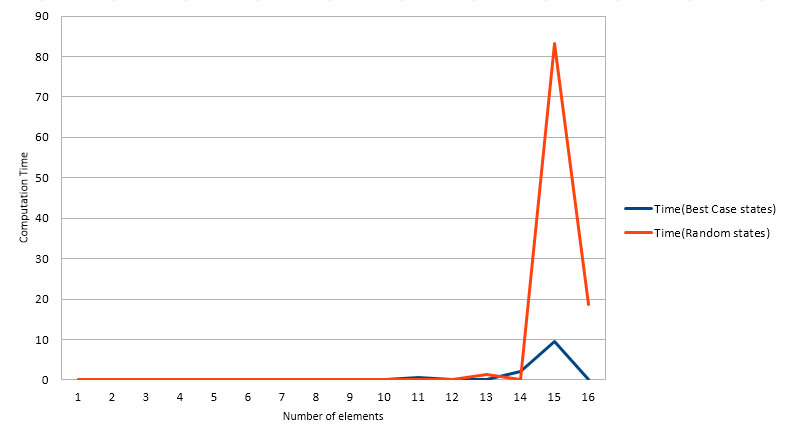
\includegraphics[width=.90\textwidth,scale=.90]{images/Recursive}
	\caption{Timed Results of Number of Pegs Versus Completion Time for Recursive Implementation}
\end{figure}

\begin{figure}[H]
	\centering
	\label{avgnumpegs}
	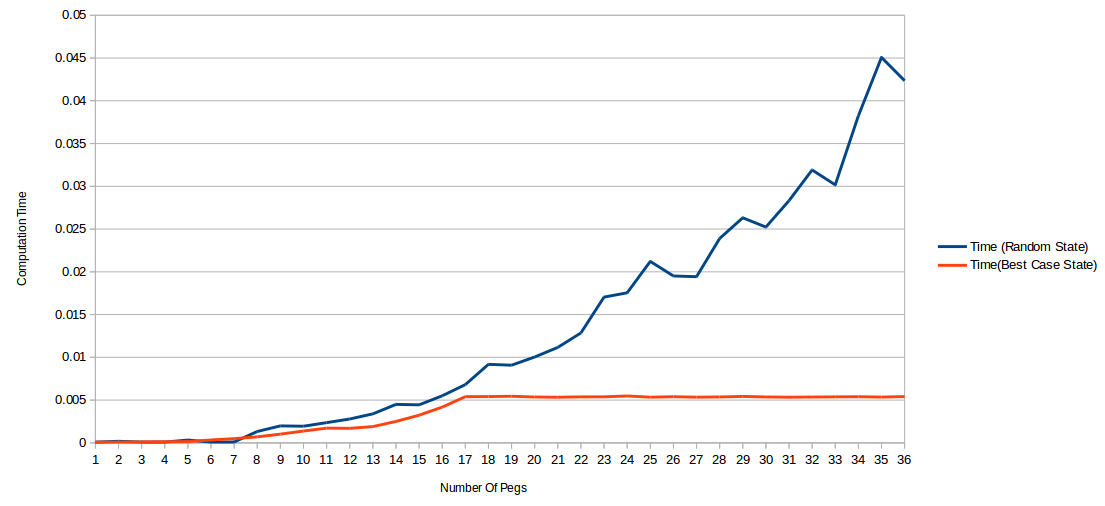
\includegraphics[width=.90\textwidth,scale=.90]{images/Stack}
	\caption{Timed Results of Number of Pegs Versus Completion Time for Stack Implementation}
\end{figure}

\begin{figure}[H]
	\centering
	\label{avgnumpegs}
	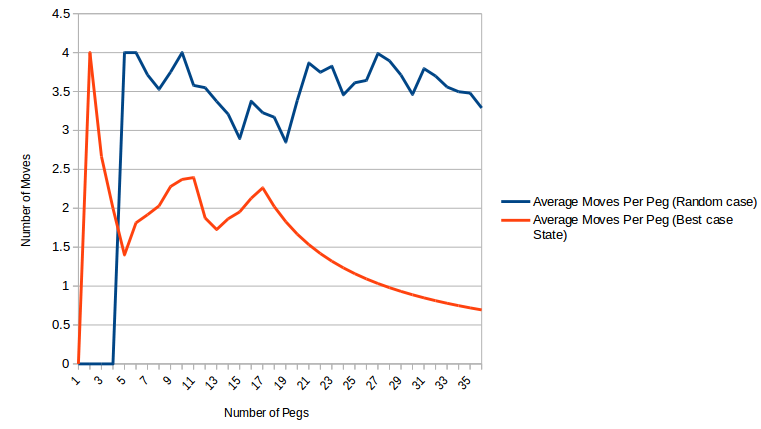
\includegraphics[width=.90\textwidth,scale=.90]{images/AverageNumPegs}
	\caption{Average Available Moves Per Peg at Each Iteration of Stack Based Algorithm}
\end{figure}

\section{Empirical Analysis}
The empirical results are shown to be within our calculated bounds (best and worst case complexities). The recursive implementation has many draw backs such as being incredibly slow and in-efficient in terms of computation and memory use. This makes the results hard to interpret. The graph does show a trend which could be described as exponential as with each step (number of initial pegs) the time difference from the last step is great. The recursive version replicates the memory state of the previous recursive step so this kind of performance is expected within c++ as recursion using the heap is not recommended for this kind of large scale state-space search \cite{bronson2012}.\\\

\noindent The stack based implementation shows a potentially exponential graph for its random case and a linear graph for its best case. The linear graph is expected as the algorithm makes use of optimized library classes such as the c++ vector \cite{bronson2012}. The random (or approximate average) graph is bounded between the two calculated theoretical complexities and so is feasible. The trend of the graph is hard to determine because of how shifted to the right it is. This graph could be exponential or even somewhat quadratic. It is most likely exponential due to the average number of pegs graph \ref{avgnumpegs} showing that for this graph the average number of pegs remains between 3 and 4 so the graph most likely reflects this branching factor. A factor of 4 is enough to shift the graph to the right in a noticeable way. \\\

\noindent The position of the initial configurations for the board plays an important role in our results. There are many configurations that are possible but from our experience in running the experiments very few initial configurations will lead to found solutions (win states). This means that the placement of pegs will have an affect on the number and size of the paths which will exist for any given game. This directly effects the time and space complexity. \\\

\noindent Our recursive implementation was very slow. An observation was made that many of the sub states of the games being simulated are not unique states. One issue discussed is that the branches found within a game are mutually exclusive since they are based on decisions (moves) that have been made. This does not mean sub-states are unique since the game board is relatively small, discrete and bounded.  A mixture of hashing tables and dynamic programming could be used to speed up the played games and make them more efficient by not repeating the same sub-calculations multiple times. This could be done by storing past calculated game-states which may occur more than some threshold amount of times. This will increase memory usage but reduce overall computational time.

\section{Conclusion}
Peg-solitaire is a game whose solutions are well suited to the backtracking algorithm because of the branching nature of the moves found in the game. Its game states are however quite complex due to the factorial nature of the board placements. The game's results are highly dependant on the initial configuration of the board and the time taken by the backtracking algorithm to find a solution or to terminate has quite a large bounded area due to the non-deterministic nature of knowing how deep a path is or if an initial setup will have a win state.  


\section{Group Member Contribution}
\begin{table}[H]
\centering
\label{contribution}
\begin{tabular}{|l|l|l|}
\hline
\textbf{Member}         & \textbf{Evan Bancroft 879192} & \textbf{Jason Chalom 711985} \\ \hline
Game                    & 75\%                          & 25\%                         \\ \hline
Back Tracking Algorithm & 50\%                          & 50\%                         \\ \hline
% Complexity Analysis     & \%                          & \%                         \\ \hline
Report                  & 25\%                          & 75\%                         \\ \hline
\end{tabular}
\caption{Contributions of Group Members By Task}
\end{table}

\section*{Acknowledgements}
All drawn diagrams were drawn using \url{http://draw.io/} and charts were made with Libre Office.\\ 
All the programming was done in c++ using OpenMP for its timing functions.\\
The lecture on backtracking and our consultation helped us to analyse our results in a meaningful way.

\bibliographystyle{plain}
\bibliography{biblio}{}
\break

\section*{Appendix A: Source Code}

% Source: backtracking.cpp
\subsection{{Source: backtracking.cpp}}
\lstinputlisting[language=C++]{../src/backtracking.cpp}

\subsection{{Source: solitaire\_board.h}}
\lstinputlisting[language=C++]{../src/solitaire_board.h}

\subsection{{Source: move.h}}
\lstinputlisting[language=C++]{../src/move.h}

\subsection{{Source: main.cpp}}
\lstinputlisting[language=C++]{../src/main.cpp}

\subsection{{Source: helpers.cpp}}
\lstinputlisting[language=C++]{../src/helpers.cpp}

\break
\section*{Appendix B: Results}

\begin{table}[H]
\centering
\label{recursive-table}
\begin{tabular}{|l|l|l|l|l|}
\hline
\textbf{Amount} & \textbf{Time(Best Case states)} & \textbf{Time(Random states)} & \textbf{Found A Path?} & \textbf{End State} \\ \hline
\textbf{1}      & 0,000012993                     & 0,000007902                  & 0                      & 3                  \\ \hline
\textbf{2}      & 0,000013994                     & 0,000007642                  & 0                      & 3                  \\ \hline
\textbf{3}      & 0,000014695                     & 0,00000827                   & 0                      & 3                  \\ \hline
\textbf{4}      & 0,000045349                     & 0,000008324                  & 0                      & 3                  \\ \hline
\textbf{5}      & 0,000017047                     & 0,00006715                   & 0                      & 3                  \\ \hline
\textbf{6}      & 0,000017154                     & 0,000045409                  & 0                      & 3                  \\ \hline
\textbf{7}      & 0,000035677                     & 0,000019492                  & 0                      & 3                  \\ \hline
\textbf{8}      & 0,000136504                     & 0,000223362                  & 0                      & 3                  \\ \hline
\textbf{9}      & 0,000953186                     & 0,00031693                   & 0                      & 3                  \\ \hline
\textbf{10}     & 0,0377231                       & 0,0249256                    & 0                      & 3                  \\ \hline
\textbf{11}     & 0,578075                        & 0,000131526                  & 0                      & 3                  \\ \hline
\textbf{12}     & 0,165076                        & 0,00613507                   & 0                      & 3                  \\ \hline
\textbf{13}     & 0,00160808                      & 1,3081                       & 0                      & 3                  \\ \hline
\textbf{14}     & 2,05269                         & 0,00337623                   & 0                      & 3                  \\ \hline
\textbf{15}     & 9,56415                         & 83,1621                      & 1                      & 3                  \\ \hline
\textbf{16}     & 0,228359                        & 18,762                       & 0                      & 3                  \\ \hline
\textbf{17}     & 314,24                          & 2442,48                      & 0                      & 3                  \\ \hline
\end{tabular}
\caption{Timed Results of Recursive Implementation}
\end{table}

\begin{table}[H]
\centering
\label{stack-table}
\begin{tabular}{|l|l|l|l|}
\hline
\textbf{Amount} & \textbf{Path Size} & \textbf{Time (Random State)} & \textbf{Time(Best Case State)} \\ \hline
\textbf{1}      & 0                  & 0,000087546                  & 0,000079554                    \\ \hline
\textbf{2}      & 1                  & 0,000180635                  & 0,000087919                    \\ \hline
\textbf{3}      & 2                  & 0,000088643                  & 0,000111731                    \\ \hline
\textbf{4}      & 3                  & 0,000089779                  & 0,000135486                    \\ \hline
\textbf{5}      & 4                  & 0,000326819                  & 0,000147682                    \\ \hline
\textbf{6}      & 6                  & 0,000095684                  & 0,000334714                    \\ \hline
\textbf{7}      & 8                  & 0,000097001                  & 0,000492098                    \\ \hline
\textbf{8}      & 9                  & 0,00132629                   & 0,000701262                    \\ \hline
\textbf{9}      & 10                 & 0,00198162                   & 0,00102037                     \\ \hline
\textbf{10}     & 11                 & 0,00194504                   & 0,00138001                     \\ \hline
\textbf{11}     & 12                 & 0,00236243                   & 0,00171943                     \\ \hline
\textbf{12}     & 14                 & 0,00278941                   & 0,0016969                      \\ \hline
\textbf{13}     & 15                 & 0,00338771                   & 0,00189975                     \\ \hline
\textbf{14}     & 16                 & 0,00449822                   & 0,00250172                     \\ \hline
\textbf{15}     & 18                 & 0,00444476                   & 0,00323355                     \\ \hline
\textbf{16}     & 19                 & 0,00549958                   & 0,00417548                     \\ \hline
\textbf{17}     & 20                 & 0,00680899                   & 0,00539972                     \\ \hline
\textbf{18}     & 20                 & 0,00917923                   & 0,00540915                     \\ \hline
\textbf{19}     & 20                 & 0,00908114                   & 0,00544882                     \\ \hline
\textbf{20}     & 20                 & 0,010037                     & 0,00536063                     \\ \hline
\textbf{21}     & 20                 & 0,0111601                    & 0,00533272                     \\ \hline
\textbf{22}     & 20                 & 0,0128546                    & 0,00537615                     \\ \hline
\textbf{23}     & 20                 & 0,0170417                    & 0,00538194                     \\ \hline
\textbf{24}     & 20                 & 0,0175451                    & 0,00548215                     \\ \hline
\textbf{25}     & 20                 & 0,0212161                    & 0,00533657                     \\ \hline
\textbf{26}     & 20                 & 0,0195111                    & 0,00539675                     \\ \hline
\textbf{27}     & 20                 & 0,0194284                    & 0,00534268                     \\ \hline
\textbf{28}     & 20                 & 0,0238981                    & 0,00536282                     \\ \hline
\textbf{29}     & 20                 & 0,0263172                    & 0,00542806                     \\ \hline
\textbf{30}     & 20                 & 0,0252291                    & 0,00536498                     \\ \hline
\textbf{31}     & 20                 & 0,0283234                    & 0,00533903                     \\ \hline
\textbf{32}     & 20                 & 0,0319084                    & 0,00535362                     \\ \hline
\textbf{33}     & 20                 & 0,030172                     & 0,00537846                     \\ \hline
\textbf{34}     & 20                 & 0,0382437                    & 0,0053947                      \\ \hline
\textbf{35}     & 20                 & 0,0450741                    & 0,0053488                      \\ \hline
\textbf{36}     & 20                 & 0,0423465                    & 0,00541166                     \\ \hline
\end{tabular}
\caption{Timed Results of Stack Based Implementation}
\end{table}

\begin{table}[]
\centering
\label{avg-pegs-table}
\begin{tabular}{|l|l|l|}
\hline
\textbf{Amount} & \textbf{Average Moves Per Peg (Random case)} & \textbf{Average Moves Per Peg (Best case State)} \\ \hline
\textbf{1}      & 0                                            & 0                                                \\ \hline
\textbf{2}      & 0                                            & 4                                                \\ \hline
\textbf{3}      & 0                                            & 2,66667                                          \\ \hline
\textbf{4}      & 0                                            & 2                                                \\ \hline
\textbf{5}      & 4                                            & 1,4                                              \\ \hline
\textbf{6}      & 4                                            & 1,8125                                           \\ \hline
\textbf{7}      & 3,71429                                      & 1,91667                                          \\ \hline
\textbf{8}      & 3,52941                                      & 2,0303                                           \\ \hline
\textbf{9}      & 3,75                                         & 2,27907                                          \\ \hline
\textbf{10}     & 4                                            & 2,37037                                          \\ \hline
\textbf{11}     & 3,57895                                      & 2,39394                                          \\ \hline
\textbf{12}     & 3,5493                                       & 1,875                                            \\ \hline
\textbf{13}     & 3,37349                                      & 1,72632                                          \\ \hline
\textbf{14}     & 3,20833                                      & 1,86486                                          \\ \hline
\textbf{15}     & 2,89655                                      & 1,95349                                          \\ \hline
\textbf{16}     & 3,375                                        & 2,12838                                          \\ \hline
\textbf{17}     & 3,22759                                      & 2,2619                                           \\ \hline
\textbf{18}     & 3,16981                                      & 2,02128                                          \\ \hline
\textbf{19}     & 2,85057                                      & 1,82692                                          \\ \hline
\textbf{20}     & 3,38798                                      & 1,66667                                          \\ \hline
\textbf{21}     & 3,86667                                      & 1,53226                                          \\ \hline
\textbf{22}     & 3,74775                                      & 1,41791                                          \\ \hline
\textbf{23}     & 3,8247                                       & 1,31944                                          \\ \hline
\textbf{24}     & 3,45763                                      & 1,23377                                          \\ \hline
\textbf{25}     & 3,6129                                       & 1,15854                                          \\ \hline
\textbf{26}     & 3,64308                                      & 1,09195                                          \\ \hline
\textbf{27}     & 3,98834                                      & 1,03261                                          \\ \hline
\textbf{28}     & 3,89474                                      & 0,979381                                         \\ \hline
\textbf{29}     & 3,71163                                      & 0,931373                                         \\ \hline
\textbf{30}     & 3,46309                                      & 0,88785                                          \\ \hline
\textbf{31}     & 3,79381                                      & 0,848214                                         \\ \hline
\textbf{32}     & 3,69925                                      & 0,811966                                         \\ \hline
\textbf{33}     & 3,55862                                      & 0,778689                                         \\ \hline
\textbf{34}     & 3,49762                                      & 0,748031                                         \\ \hline
\textbf{35}     & 3,47977                                      & 0,719697                                         \\ \hline
\textbf{36}     & 3,28937                                      & 0,693431                                         \\ \hline
\end{tabular}
\caption{Average Available Moves Per Peg for the Stack Implementation}
\end{table}

\end{document}